\section{Info-Dialog Plug-Ins}
	  This class provides a minor extension of standard dialog plug-ins. The main difference is that the dialogs have only informational purpose but cannot be used to save modified data at the server. The specified dialogs are shown as tabs below the editor (see Figure \ref{info_dialog_screenshot}). Except for \verb!saveData()!, the implementer has to implement the same methods as for dialog plug-ins (cf. Section \ref{dialog_plugins}).

	\begin{figure}[ht]
	  \centering
	  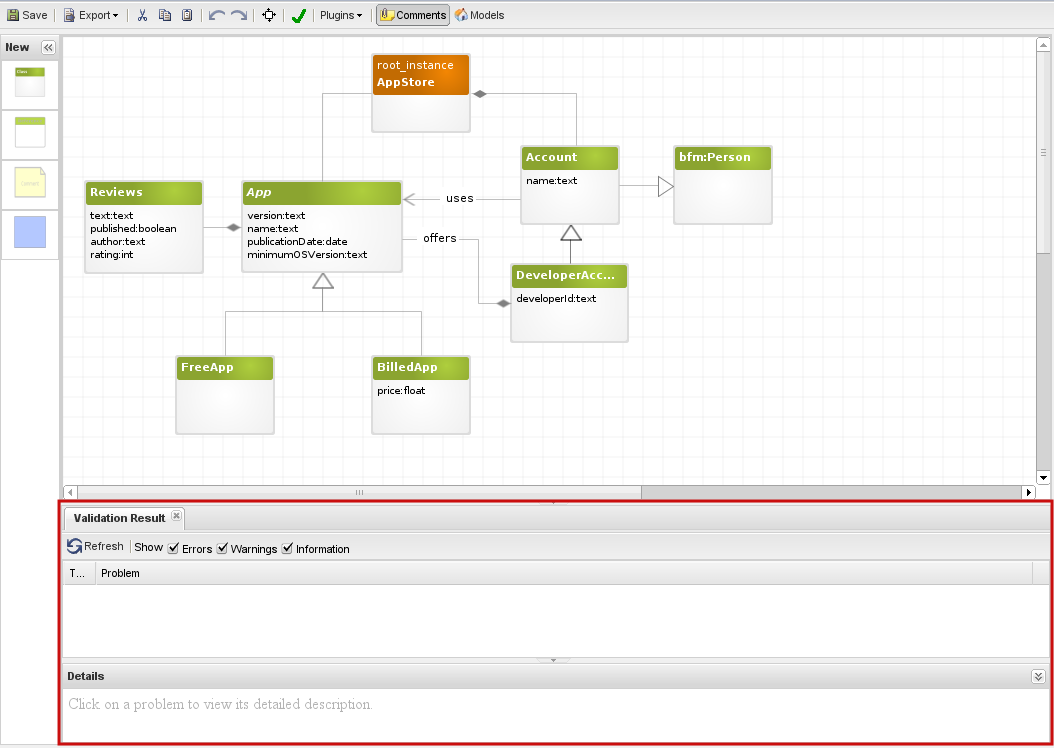
\includegraphics[width=0.8\textwidth]{graphics/info_dialog_screenshot}
	  \caption{Display area for info-dialog plug-ins}
	  \label{info_dialog_screenshot}
	\end{figure}

	\subsection{JavaScript}
	In contrast to standard dialog plug-ins, the main JavaScript class has to inherit from \verb!Ext.ux.InfoDialog!, which is itself an extension of \verb!Ext.ux.Dialog!. Listing \ref{infodialog_js} displays the source code of \verb!Ext.ux.InfoDialog!. As one can see, the dialog has access to the plug-in it is created for. Thereby, the dialog is able to refresh the displayed data by calling \verb!this.plugin.refreshData()!. This refresh mechanism can be used ,e.g., to implement a refresh button.
	\clearpage
	\begin{lstlisting}[language=Java, caption=Ext.ux.Dialog, label=infodialog_js]
Ext.namespace("Ext.ux");

Ext.ux.InfoDialog = Ext.extend( Ext.ux.Dialog, {
    constructor : function( config ) {
        Ext.ux.InfoDialog.superclass.constructor.call(this, config);
    },

    setPlugin : function( plugin ) {
        this.plugin = plugin;
    }
});
	\end{lstlisting}
	